\section*{Assignment 05: Governance and Data Policies}
\addcontentsline{toc}{section}{Assignment 05: Governance and Data Policies}

\subsection*{Onboarding and moderation architecture}
I combined \citet{Choudary2016}'s participation formula with \citet{Reillier2017}'s governance levers to draft the onboarding and moderation plan. Participation requires access, ability, and incentive. Access comes from institution issued logins for students and invitation codes for NGOs. Ability is supported by guided tours, examples, and a first mission checklist. Incentive arrives through portfolio boosts for students and impact dashboards for organisations.

The onboarding journey unfolds in three concrete steps. First, \textbf{a welcome screen} previews sample projects and spells out expectations. Second, \textbf{profile setup} uses defaults for skills, availability, and preferred communication styles. Third, the \textbf{first mission checklist} unlocks only after users read the code of conduct and complete a practice task. Each step ends with a short micro survey so the team collects immediate feedback, reflecting Lecture~5's reminder to treat onboarding as an experiment \citep{Lecture05}.

Moderation uses a layered structure based on \citet{Choudary2016}'s categories of prevention, detection, and enforcement. Automated filters remove clear spam. Community stewards, made up of experienced students and NGO staff, can hide content for a short time and ask for review. A professional response team handles serious cases within twenty four hours, using playbooks created with NGO advisors. Training includes de escalation scripts because previous cases showed that many NGOs work with vulnerable groups, and poor communication can retraumatise participants \citep{Lecture11}. Quarterly tabletop drills check that the process remains effective.

\subsection*{Data policy and transparency}
Data collection follows the \textit{minimalism principle} from \citet{Zuboff2019}. SkillSync only stores information needed for matching, payouts, and quality assurance. This includes profile basics, project actions, satisfaction scores, and optional testimonials. \textit{Advanced analytics} need clear opt in during onboarding. The default data retention period is two years unless users ask for a different duration.

Transparency is implemented through a \textit{data mirror} inside the product. Users can see every \textit{datapoint} linked to their account, download it, or delete it unless a legal hold applies. Release notes share summaries of \textit{algorithm} updates, moderation results, and incident reports every quarter. An internal \textit{ethics council} meets each month to review new experiments. This council uses \citet{Reillier2017}'s \textit{governance canvas} to check if changes shift power unfairly. External advisors from partner NGOs receive the same reports to maintain legitimacy and trust \citep{Srnicek2017}.

Figure~\ref{fig:onboarding-flow} shows the four step carousel that guides onboarding. Each panel uses simple language and includes an indicator explaining why the step is important so users do not feel misled. The design follows the \textit{show not tell} advice from Lecture~5 on metrics and instrumentation \citep{Lecture05}.

\begin{figure}[H]
  \centering
  \begin{minipage}[b]{0.45\textwidth}
    \centering
    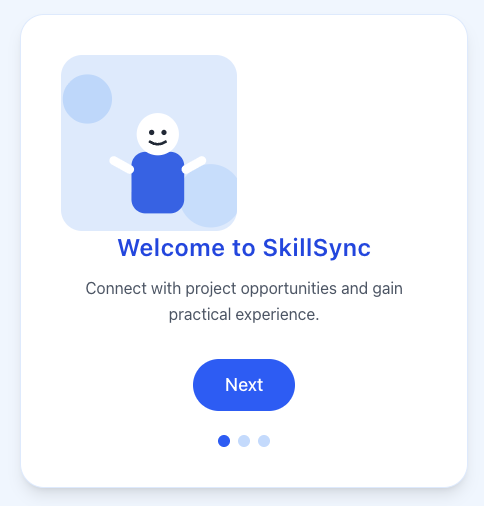
\includegraphics[width=\linewidth]{figures/Onboarding-1.png}\\[0.3em]
    
\includegraphics[width=\linewidth]{figures/Onboarding-2.png}
  \end{minipage}\hfill
  \begin{minipage}[b]{0.45\textwidth}
    \centering
    
\includegraphics[width=\linewidth]{figures/Onboarding-3.png}\\[0.3em]
    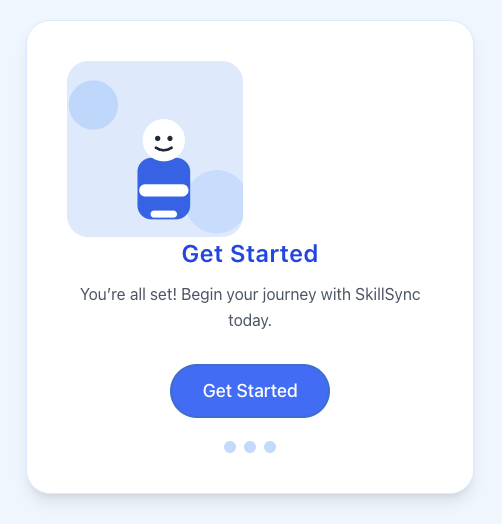
\includegraphics[width=\linewidth]{figures/Onboarding-4.png}
  \end{minipage}
  \caption{Guided onboarding carousel with four step checklist.}
  \label{fig:onboarding-flow}
\end{figure}

Governance tooling is shown in Figure~\ref{fig:admin-panel}. The administrator dashboard brings together flagged content, dispute queues, and \textit{fairness metrics} beside response time goals. Moderators can look into case history, use prewritten responses, ask for help from legal counsel, and download evidence for quarterly reports. These functions match the enforcement levers described in \citet{Reillier2017} and make accountability clear.

\begin{figure}[H]
  \centering
  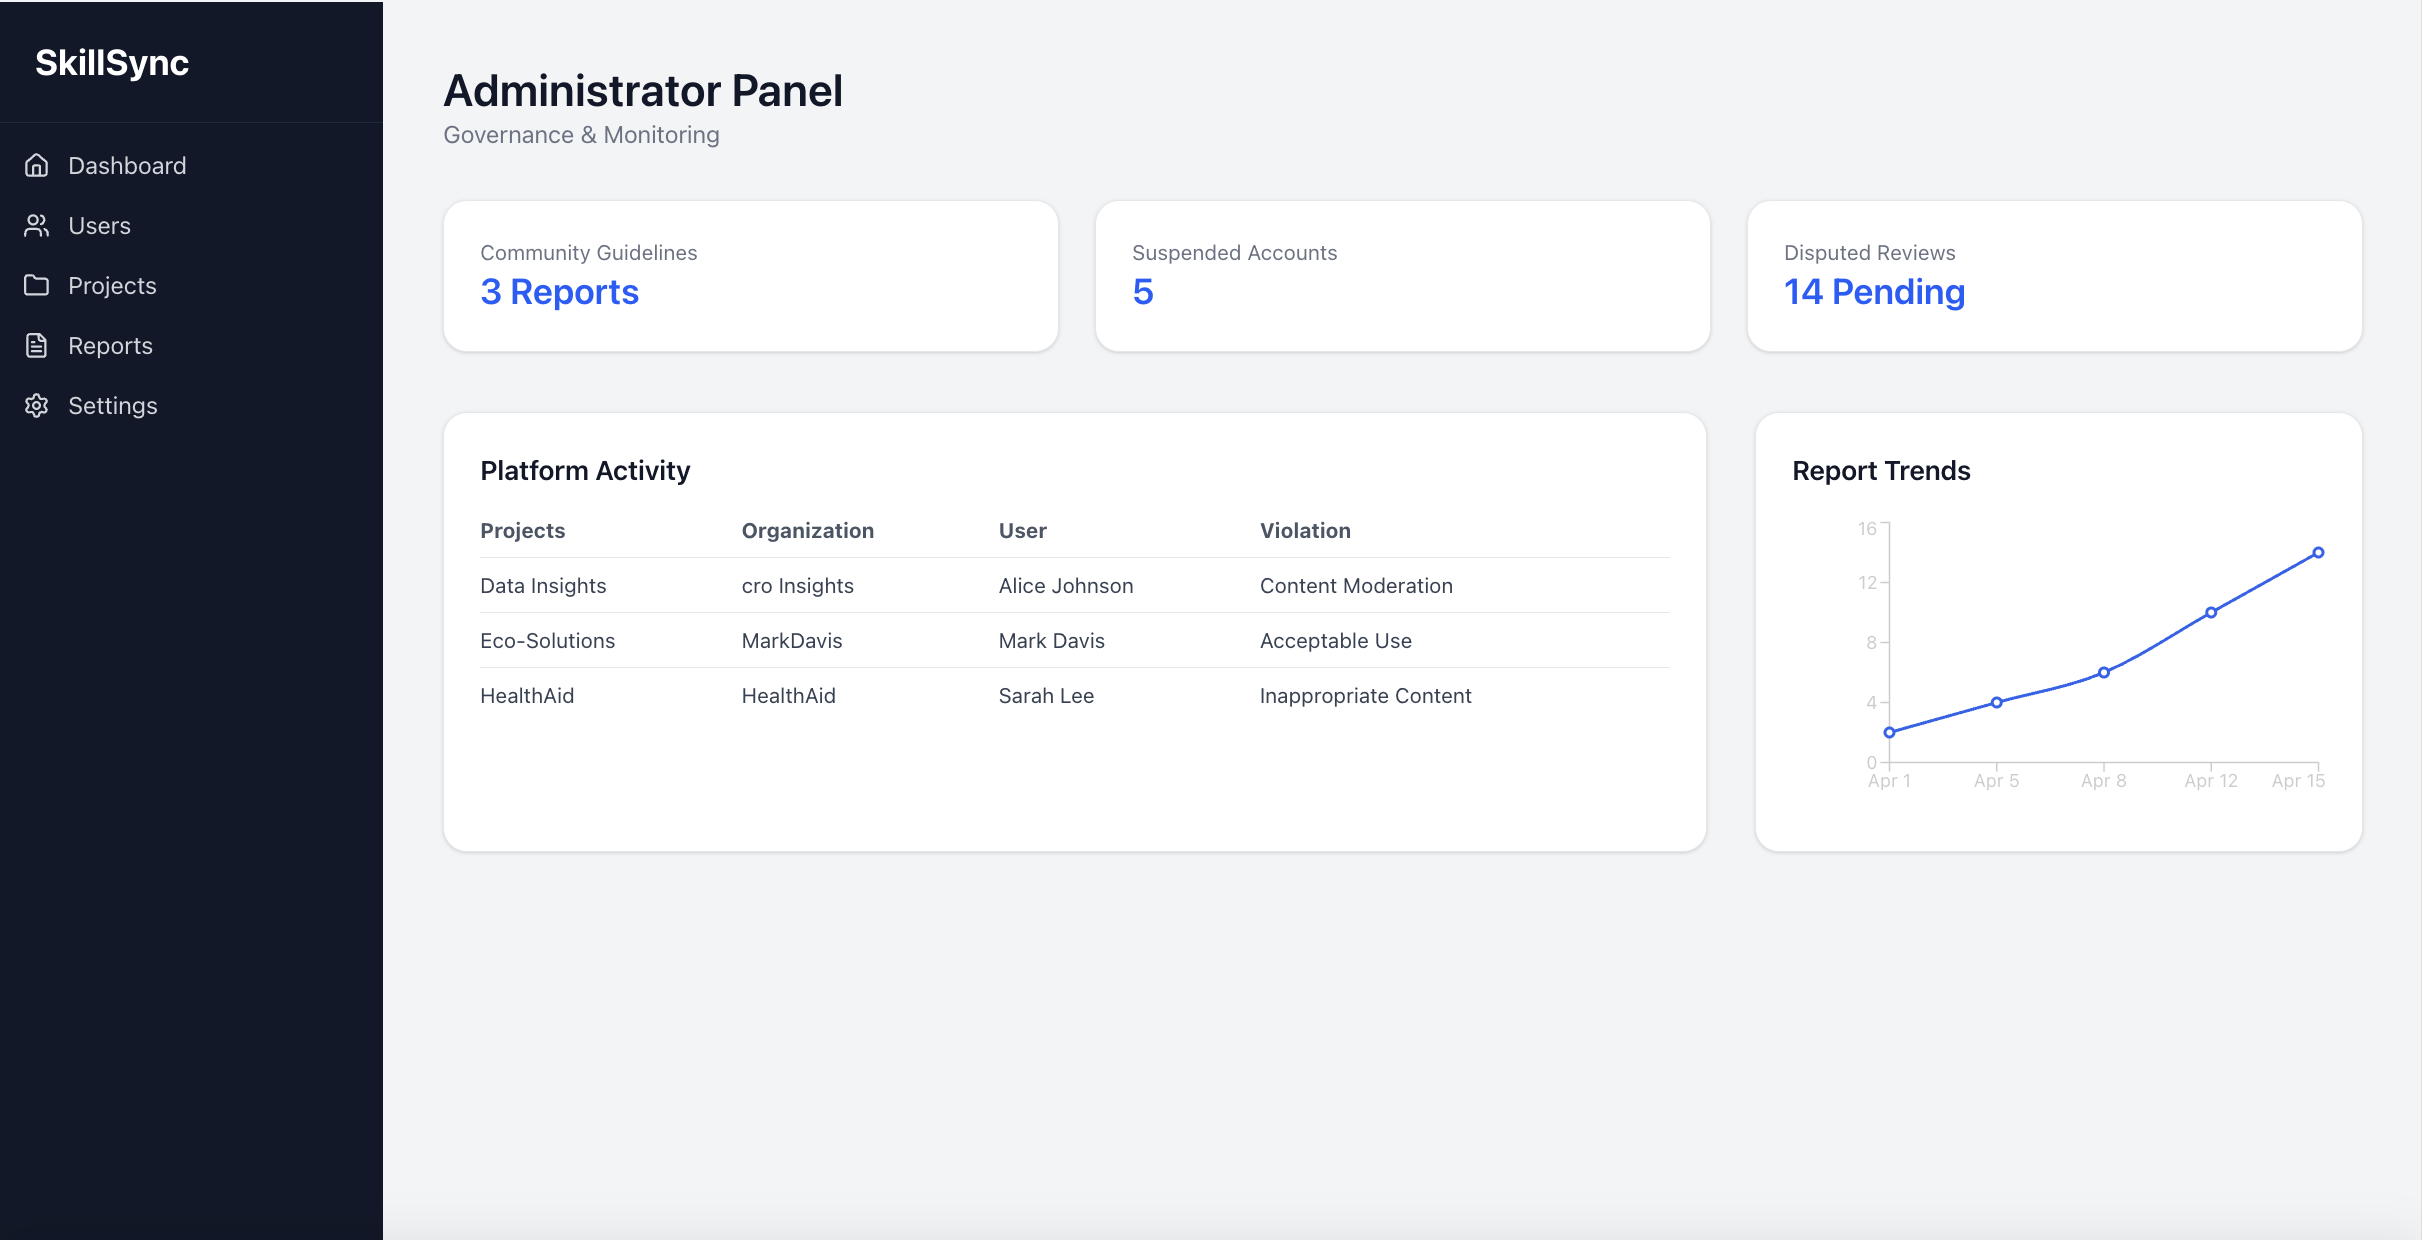
\includegraphics[width=0.85\linewidth]{figures/Organisation-Administratorpanel.png}
  \caption{Governance control room mock up with moderation and fairness metrics.}
  \label{fig:admin-panel}
\end{figure}

Finally, communication remains human. Automated nudges use friendly language and include links to policy explanations. Moderators join workshops with partner NGOs to learn about sensitive situations. Every three months, community sessions let experienced users question the product team before big updates. This follows Lecture~11’s idea of building legitimacy through dialogue \citep{Lecture11}.
